\section{Objective 26}
\subsection{}
\frame{\sectionpage}
\subsection{Terminology}
\frame{\subsectionpage}
\begin{frame}{Definitions}
    \begin{itemize}
        \item<1->{A \textcolor{orange}{\textbf{vector-valued equation}} is an equation that expresses a vector in terms of a parameter.}
        \item<2->{A \textcolor{orange}{\textbf{line}} is a straight path that extends infinitely in two directions.}
        \item<3->{\textcolor{orange}{\textbf{Three-dimensional space}} is the space in which three coordinates are needed to specify a point.}
    \end{itemize}
\end{frame}
\subsection{Objective Defined}
\frame{\subsectionpage}
\begin{frame}{What is Objective 26?}
    \begin{block}{Objective Definition}
        In this objective, you must be able to... \\
        \color{orange}{``Write the vector-valued equation of a line in three dimensions.``}
    \end{block}
\end{frame}
\begin{frame}{But what does that mean?}
    \begin{itemize}
        \item<1-2>{Well, in baby terms...}
        \begin{itemize}
            \item<2>{We want to write an equation that tells us where a line is in 3D space.}
        \end{itemize}
    \end{itemize}
\end{frame}
\subsection{\textit{Modus Operandi}}
\frame{\subsectionpage}
\begin{frame}{Formula}
    \begin{block}{Formula}
        A line in three dimensions can be defined by a vector-valued equation
        \begin{align*}
            \vec{r}(t) = r_0 + t \vec{v}
        \end{align*}
    \end{block}
\end{frame}
\begin{frame}{Formula}
    \begin{block}{Formula (cont.)}
        Where:
        \begin{itemize}
            \item<2->{\begingroup\color{orange}{\bm{$\vec{r}(t)$}}\endgroup \ is the vector-valued equation of the line.}
            \item<3->{\begingroup\color{orange}{\bm{$r_0$}}\endgroup \ is the starting point of the line.}
            \item<4->{\begingroup\color{orange}{\bm{$t$}}\endgroup \ is the parameter used to determine the position of any point on the line.}
            \item<5>{\begingroup\color{orange}{\bm{$\vec{v}$}}\endgroup \ is the direction vector of the line.}
        \end{itemize}
    \end{block}
\end{frame}
\subsection{Explanation}
\frame{\subsectionpage}
\begin{frame}{Explanation}
    \uncover<1->{\textbf{So, what was all of that?}}
    \begin{itemize}
        \item<2->{By using a vector-valued equation with a parameter \begingroup\color{orange}{\bm{$t$}}\endgroup , we can represent any point on the line by substituting different values of \begingroup\color{orange}{\bm{$t$}}\endgroup \ into the equation.}
        \item<3->{The direction vector \begingroup\color{orange}{\bm{$\vec{v}$}}\endgroup \ determines the slope of the line, and the starting point \begingroup\color{orange}{\bm{$a$}}\endgroup \ determines where the line begins.}
    \end{itemize}
\end{frame}
\subsection{Example}
\frame{\subsectionpage}
\begin{frame}{Example}
    \textbf{Example}
    \begin{block}{Problem}
        \textbf{What is the vector equation of a line that passes through the points (2, 4, -3) and (4, 1, 5)?}
    \end{block}
\end{frame}
\begin{frame}{Example}
    \textbf{First, we need to find the direction vector. Let point (2, 4, -3) equal \begingroup\color{orange}{\bm{$A$}}\endgroup \ and point   equal \begingroup\color{orange}{\bm{$B$}}\endgroup :}
    \begin{align*}
        \uncover<2->{\vec{AB} = \langle 4-2, 1-4, 5-(-3) \rangle} \\
        \uncover<3->{= \langle 2, -3, 8 \rangle}
    \end{align*}
\end{frame}
\begin{frame}{Example}
    \textbf{Now, we need to get the starting point, or \begingroup\color{orange}{\bm{$r_0$}}\endgroup .} \\
    \uncover<2->{\textbf{Since we chose \begingroup\color{orange}{\bm{$A$}}\endgroup \ to be the initial point of \begingroup\color{orange}{\bm{$\vec{AB}$}}\endgroup , we can just use the coordinates of  \begingroup\color{orange}{\bm{$A$}}\endgroup \ as  \begingroup\color{orange}{\bm{$r_0$}}\endgroup .}}
    \begin{align*}
        \uncover<3->{r_0 = (2, 4, -3)}
    \end{align*}
\end{frame}
\begin{frame}{Example}
    \textbf{Now, we can put it all together:}
    \begin{align*}
        \uncover<2->{r = r_0 + t \vec{v}} \\
        \uncover<3->{r_0 = (2, 4, -3)} \\
        \uncover<4->{\vec{v} = \vec{AB} = \langle 2, -3, 8 \rangle} \\
        \uncover<5->{r = \langle 1+3t, 3-2t, -2+7t \rangle} \\
    \end{align*}
    \uncover<6->{\textbf{We could have also done it in the opposite direction as long as we set \begingroup\color{orange}{\bm{$r_0$}}\endgroup \ to be \begingroup\color{orange}{\bm{$B$}}\endgroup \ and set \begingroup\color{orange}{\bm{$v$}}\endgroup \ to be \begingroup\color{orange}{\bm{$\vec{BA}$}}\endgroup.}}
\end{frame}
\begin{frame}{Example}
    \textbf{A substandard visual}
    \uncover<2->{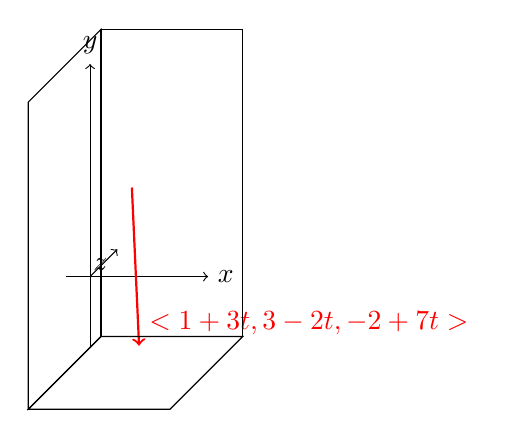
\begin{tikzpicture}[scale=0.3]
        % Set axis limits
        \draw[->] (-1,0) -- (5,0) node[right] {$x$};
        \draw[->] (0,-3) -- (0,9) node[above] {$y$};
        \draw[->] (0,0) -- (0,0,-3) node[below left] {$z$};
        
        % Plot vector equation
        \draw[red,thick,->] (1,3,-2) -- (4,-1,5) node[above right] {$<1+3t, 3-2t, -2+7t>$};
        
        % Adjust axis limits
        \pgfmathsetmacro{\xmax}{5.5}
        \pgfmathsetmacro{\ymax}{9.5}
        \pgfmathsetmacro{\zmax}{5.5}
        \pgfmathsetmacro{\xmin}{-0.5}
        \pgfmathsetmacro{\ymin}{-3.5}
        \pgfmathsetmacro{\zmin}{-2.5}
        \draw (\xmin,\ymin,\zmin) -- (\xmax,\ymin,\zmin) -- (\xmax,\ymax,\zmin) -- (\xmin,\ymax,\zmin) -- cycle;
        \draw (\xmin,\ymin,\zmin) -- (\xmin,\ymin,\zmax) -- (\xmin,\ymax,\zmax) -- (\xmin,\ymax,\zmin) -- cycle;
        \draw (\xmin,\ymin,\zmin) -- (\xmin,\ymin,\zmax) -- (\xmax,\ymin,\zmax) -- (\xmax,\ymin,\zmin) -- cycle;
        
        \end{tikzpicture}}
\end{frame}
\subsection{Objective Summary}
\frame{\subsectionpage}
\begin{frame}{Objective Summary}
    \textbf{To write the vector-valued equation of a line in three dimensions:}
    \begin{itemize}
        \item<2->{Find the direction vector.}
        \item<3->{Find the starting point.}
        \item<4->{Write the vector-valued equation.}
    \end{itemize}
    \uncover<5->{\textbf{Remember:} \textit{The direction vector determines the slope of the line, and the starting point determines where the line begins.}}
\end{frame}
